\section{Structural Theory }

\subsection{Neural Network}

    A Neural Network (NN) is a computational model inspired by the structure and functioning of biological neural networks found in the human brain. It is a cornerstone of machine learning, particularly excelling in tasks that involve pattern recognition, data classification, and function approximation. Neural networks are composed of interconnected layers of nodes, often called neurons or perceptrons, designed to process and transform data through mathematical operations.

The fundamental building block of a neural network is the artificial neuron, which performs a weighted sum of inputs followed by a nonlinear activation function. These neurons are organized into layers:

\textbf{Input Layer:} Receives raw data or features for processing.

\textbf{Hidden Layers:} Perform transformations to capture patterns and abstractions.

\textbf{Output Layer:} Produces the final result, such as a prediction or classification.
A neural network learns to map inputs to outputs by adjusting the weights of its connections through an optimization process called training. Training involves minimizing a predefined loss function that quantifies the difference between the predicted output and the actual target. This is typically achieved using algorithms like gradient descent and its variants.

Compared with Linear Regression and Logistic Regression, Neutral Network is a Regression model that eliminated the effects of Linearity relationship through Activations models and multiple layer of relationship, moreover, Neutral Network analyse deeper relationship than Logistic Regression, however, unlike Logistic Regression, the Neutral Network is a \textbf{Black-box model}, meaning we are un-likely to know how it is truely trains if the model is large, this may create a \textbf{Gradient Dissapear} and \textbf{Overfitting} of trainned nodes, which can be partly eliminate through \textbf{Dropout}

Similar to Logistic Regression, each Node of Neutral Networks is actually a Logistic Regression, with \textbf{Linear Layer} and corresponding \textbf{Activate Function} (Sigmoid for Logistic Regression) for Linearity removal and Binary transformations

% \subsubsubsection*{Forward Propagation (Inference)}

%%%%%%%%%%%%%%%%%%%%%%%%%%%

\subsection{Convolutional Neural Networks (CNN)}

In the early days of Computer Vision, most of the approaches focus on Feature Extraction using Un-Supervised Machine Learning combine with   classification such as SVM or Neutral Networks to classify the pictures labels, however, it is not possible for Segmentational and Object Detection due to the computational problems and feature extractions, take example for a 64x64x3 pictures, if we use traditional feature extractions, let assume it is 32x32x6 using PCA, then we have to input the total of 12288 Input Nodes, for this we want to consider for more, control-able ways and faster computations.

Convolutional Neural Networks (CNNs) are a class of deep learning models specifically designed for processing data with a grid-like structure, such as images and time-series data. CNNs exploit the spatial and temporal hierarchies in data, making them highly effective for tasks like image recognition, object detection, and natural language processing. The core building block of a CNN is the \textit{convolution operation}, which applies a filter (or kernel) to an input to extract local patterns. Mathematically, for a 2D input \( I(x, y) \) and a kernel \( K(u, v) \),  in realistic application, the CNNs mostly contructed using cross-correlation, which is faster in computations time:

\[
S(x, y) = \sum_{u}\sum_{v} I(x + u, y + v) \cdot K(u, v)
\]

Following the convolutional layer, a Pooling Layer is often applied, which extracts the importance information of a regions of Feature Map. The most common pooling operation is max-pooling, where the maximum value from a region is selected, reducing the size of the feature map while preserving important information. This helps to make the model more invariant to small translations of the image.

Finally, the fully connected layers may be appiled at the end of the network help in classification by using the features extracted from the convolutional layers and pooling layers to make predictions. The last fully connected layeruses a activation function for multi-class classification tasks, this ensurance of first-trainning predictions value not being too ambigous, as un-expected value can be the output.

\subsubsection*{Max Pooling} Max-pooling is used to reduce the spatial dimensions of the feature map by selecting the maximum value in a specified window, often $2 \times 2$. This operation helps to decrease the computational load while preserving the most important features.

\begin{align}
\text{MaxPool}(I) = \max(I)
\end{align}

Translation equivariance is a fundamental property of \textbf{Convolutional}, see figure \ref{fig:CNNs}. It refers to the idea that a shift in the input leads to a corresponding shift in the output feature map. This ensures that the spatial structure of the detected features is preserved across translations. In computer visions, positional and represented change are strongly affected the final feature map which will costly for regression steps.

\begin{figure}[h]
    \centering
    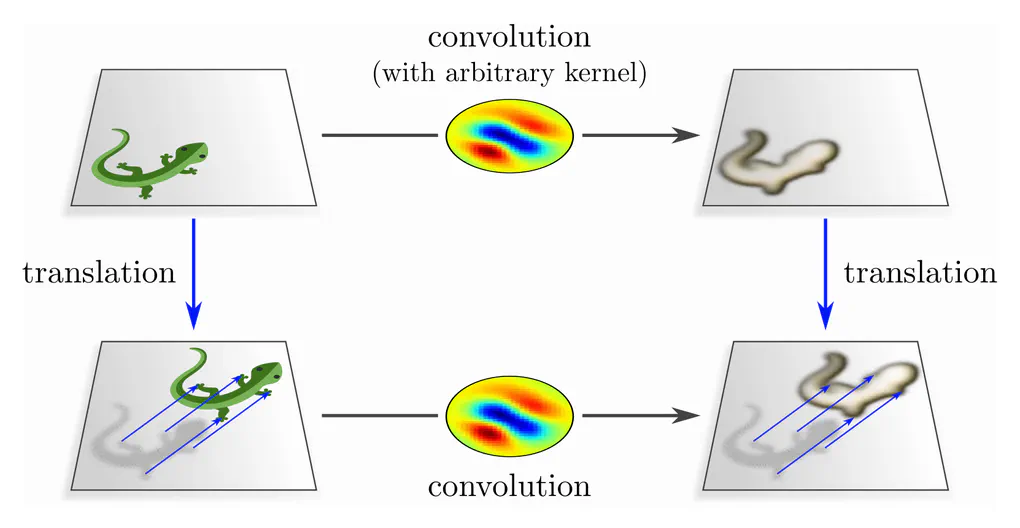
\includegraphics[width=0.5\linewidth]{theoretical-background/image/CNNs.png}
    \caption{Translation equivariance}
    \label{fig:CNNs}
\end{figure}

When max pooling is used in CNNs, it reduces the model’s sensitivity to small shifts in the input. This means that some of the precise location information can be lost and the model becomes less translation-equivariant or \textbf{ translation-inequivariant}. However, this is not mean that both equivariant and in-inequivariant can not be happen at the same time, as a result, the way objects are distributed in different positions of the image can significantly affect the model’s final predictions.

To help the model handle these variations on large and imbalance datasets in object positions, a common solution is to use data augmentation. By introducing random translations, rotations, and other transformations during training, the model learns to be more robust to changes in object locations. This helps improve its ability to generalize to different input distributions.

In summary, CNNs are a powerful class of models in deep learning that are particularly suited for image-related tasks due to their ability to learn hierarchical feature representations efficiently, it can easily learn the information , however, its poor ability to adapt globaly informations are crutial downgrade for traditional CNNs model.  

\begin{figure}[h]
    \centering
    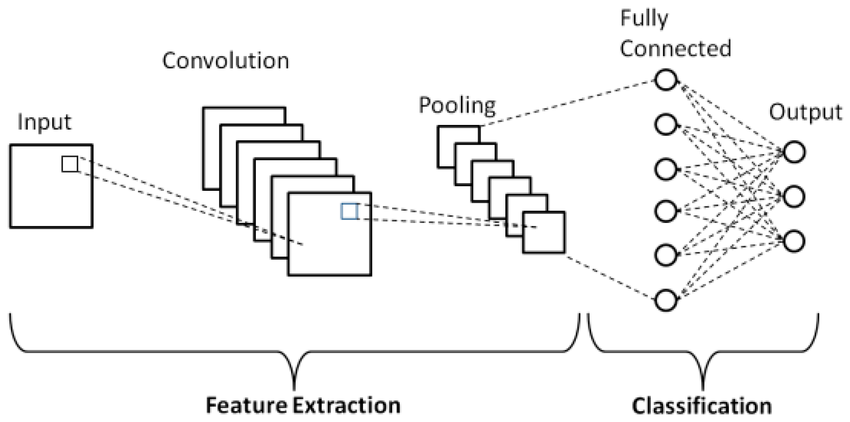
\includegraphics[width=0.5\textwidth]{theoretical-background/image/cnn.png}
    \caption{Schematic diagram of a basic Convolutional Neural Network (CNN) architecture.}
    \label{fig:cnn}
\end{figure}


% The development of Deformable Convolution have been development to limit the effections of variations and global learning problem, 

% \ref{image:deCNN} 

% \begin{figure}
%     \centering
%     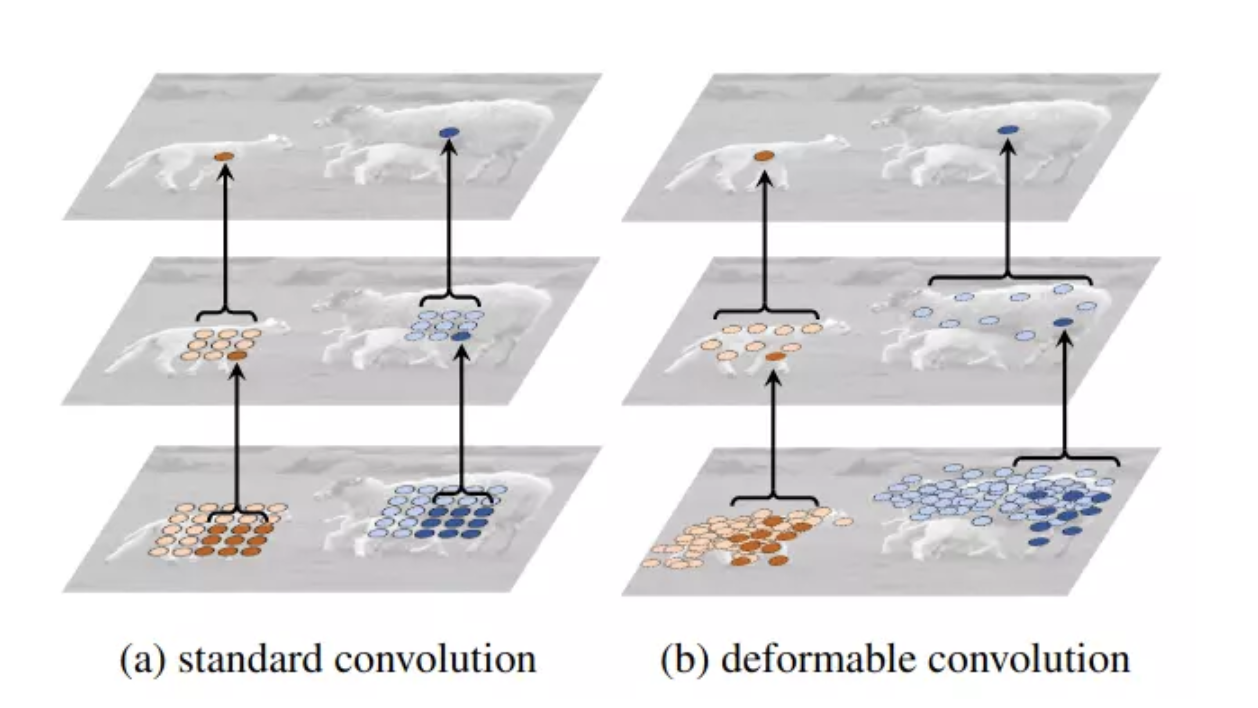
\includegraphics[width=0.5\linewidth]{theoretical-background/image/deCNN.png}
%     \caption{deformable CNN}
%     \label{fig:deCNN}
% \end{figure}


%%%%%%%%%%%%%%%%%%%%%%%%%%%%%%%%%%%%%%%%%%%%%%%%%%%%%%%%%%%%

\subsection{Positional Encoding}

Transformers lack inherent information about the order of tokens because their attention mechanism processes input tokens in parallel without considering sequence order. To enable the model to capture the relative or absolute position of tokens within a sequence, positional encoding is introduced. This encoding injects position-related information into the model, allowing it to distinguish between different token positions and thus understand the sequence structure, which is essential for tasks like language modeling and reasoning 

The most common choices for positional encoding
are either absolute, where each absolute position (e.g. 1, 2, 3, ...) is directly represented, or relative,
where the distance between tokens is used as positional information. In this section, we briefly review
the popular encoding methods used in Transformers\cite{kazemnejad2023impact}

The process of Absolute Positional Encoding (APE) involves assigning a position vector $\mathbf{p}_i$ to each absolute position $i$ and combining them with word embeddings before inputting them into the model. APE modifies how the hidden state is initialized:

\begin{equation}
\mathbf{H}^{(0)} = \mathbf{W}_E \mathbf{X} + \mathbf{W}_P \mathbf{P}
\end{equation}

where $\mathbf{W}_P \in \mathbb{R}^{d \times T}$ is the positional embedding matrix, and $\mathbf{P} \in \mathbb{R}^{V_p \times (T + 1)}$ is the one-hot encoded absolute position sequence. $V_p$ is the maximum absolute position. Therefore, the hidden state at column $j$ is:

\begin{equation}
\mathbf{h}^{(0)}_j = \mathbf{e}_j + \mathbf{p}_j
\end{equation}
where $\mathbf{e}_j \in \mathbb{R}^d$ is the word embedding of token $x_j$ and $\mathbf{p}_j \in \mathbb{R}^d$ is the positional embedding for position $j$. Then, the dot product for the first layer in Equation (6) is computed as:

\begin{align}
\langle \mathbf{q}_t, \mathbf{k}_i \rangle 
&= \langle \mathbf{W}_Q \mathbf{h}^{(0)}_t, \mathbf{W}_K \mathbf{h}^{(0)}_i \rangle \\
&= \langle \mathbf{W}_Q (\mathbf{e}_t + \mathbf{p}_t), \mathbf{W}_K (\mathbf{e}_i + \mathbf{p}_i) \rangle \\
&= (\mathbf{W}_Q (\mathbf{e}_t + \mathbf{p}_t))^\top (\mathbf{W}_K (\mathbf{e}_i + \mathbf{p}_i)) \\
&= \mathbf{e}_t^\top \mathbf{W}_Q^\top \mathbf{W}_K \mathbf{e}_i 
+ \mathbf{e}_t^\top \mathbf{W}_Q^\top \mathbf{W}_K \mathbf{p}_i \notag \\
&\quad + \mathbf{p}_t^\top \mathbf{W}_Q^\top \mathbf{W}_K \mathbf{e}_i 
+ \mathbf{p}_t^\top \mathbf{W}_Q^\top \mathbf{W}_K \mathbf{p}_i
\end{align}

In the learned variant of APE, $\mathbf{p}_j \in \mathbb{R}^d$ is learned during training. In the sinusoidal variant, $\mathbf{p}_j$ is calculated using a non-parametric function. Specifically, $\mathbf{p}_j$ is computed as:

\begin{equation}
\mathbf{p}_j = 
\begin{bmatrix}
\sin(\omega_1 j), & \cos(\omega_1 j), & \sin(\omega_2 j), & \cos(\omega_2 j), & \ldots, & \sin(\omega_{d/2} j), & \cos(\omega_{d/2} j)
\end{bmatrix}^\top
\end{equation}

where 
\begin{equation}
\omega_i = \frac{1}{10000^{2i/d}}
\end{equation}

\subsection{Attention}

The \textbf{Attention mechanism} is a fundamental component in modern deep learning architectures, particularly in natural language processing and computer vision. Originally introduced to improve sequence modeling by selectively focusing on relevant parts of the input, attention has since evolved into a versatile framework for enhancing representation learning in a variety of domains.

At its core, attention allows a model to compute a weighted combination of input features based on their relevance to a given task. Instead of treating all inputs equally, the attention mechanism dynamically assigns higher weights to more important elements, enabling the network to "attend" to informative content while suppressing irrelevant or redundant data. This capability is especially useful in scenarios involving long-range dependencies, occlusions, or cluttered visual scenes.

\subsubsection{Scaled Dot-Product Attention}It computes how much each value vector contributes to the output vector, based on the similarity between the query vector Q and the key vector Q. The similarity is measured by the dot product, which is scaled down by the square root of the dimension of the key vector $d_k$. The scaled dot products are then normalized by a softmax function to get the attention weights. The output vector is the weighted sum of the value vectors.
\begin{align}
    Attention (Q,K,V)=softmax(\frac{QK^T}{\sqrt(d_k)})V
\end{align}

\subsubsection{Multi-head Attention}It applies the attention function multiple times in parallel, each of them is called a head, using different projections of the query, key and value vectors. This allows the model to capture different aspects of the input and output sequences. The outputs of the multi-head attention are concatenated and projected to get the final output.
\begin{align}
    MultiHead(Q,K,V)= Concat(head_1,...,head_h)W^O\\
    \text{where } head_i=Attention(QW_{i}^Q, KW_{i}^K, VW_{i}^V)
\end{align}

\subsubsection{Channel Attention}
The feature maps of CNNs produced by intermediate layers consist of multiple channels, each of which is responsible for detecting certain types of patterns such as edges, textures, or semantic parts. However, not all channels are equally important for every task or input. Some channels may contribute significantly to the final prediction, while others may introduce noise or be less relevant. 

To address this issue, attention mechanisms have been research to allow networks to adaptively focus on the most informative components of the input. One such mechanism is \textbf{channel attention}, which emphasizes meaningful channels and suppresses less useful ones. This technique enables the model to learn how to dynamically adjust the importance of each channel based on the input data, enhancing its representational power. A well-known implementation of channel attention is the \textit{Squeeze-and-Excitation (SE)} block~\cite{hu2018squeeze}, which has been widely adopted due to its simplicity and effectiveness.

Let \( \mathbf{F} \in \mathbb{R}^{C \times H \times W} \) be an intermediate feature map in a CNN, where \( C \) is the number of channels, and \( H \) and \( W \) are the spatial dimensions. The goal is to compute a set of attention weights \( \mathbf{w} \in \mathbb{R}^{C} \), one for each channel, which will be used to rescale the original feature map to emphasize informative features.

\textbf{Squeeze Global Information Embedding}

The first step is to aggregate global spatial information from each channel to form a compact descriptor. This is achieved using global average pooling across the spatial dimensions. For each channel \( c \), we compute:

\[
z_c = \frac{1}{H \cdot W} \sum_{i=1}^{H} \sum_{j=1}^{W} \mathbf{F}^{(c)}(i,j)
\]

This operation results in a vector \( \mathbf{z} \in \mathbb{R}^{C} \) that captures a global representation of the feature map across channels.

\textbf{Excitation: Adaptive Recalibration of Channels}

Next, the descriptor \( \mathbf{z} \) is passed through a lightweight gating mechanism to produce channel-wise attention weights. This gating mechanism is typically implemented as a two-layer fully connected network with a non-linear activation in between:

\[
\mathbf{w} = \sigma \left( W_2 \cdot \text{ReLU}(W_1 \cdot \mathbf{z}) \right)
\]

Here, \( W_1 \in \mathbb{R}^{\frac{C}{r} \times C} \) and \( W_2 \in \mathbb{R}^{C \times \frac{C}{r}} \) are learned weight matrices of the fully connected layers, where \( r \) is a reduction ratio that controls the bottleneck dimensionality, often set to 16. The function \( \sigma(\cdot) \) denotes the sigmoid activation, which ensures that the resulting attention weights lie in the range \( (0, 1) \).

\textbf{Recalibration: Channel-wise Scaling}

Finally, the original feature map is rescaled using the learned channel weights. Each channel \( \mathbf{F}^{(c)} \) is multiplied by the corresponding scalar weight \( w_c \):

\[
\tilde{\mathbf{F}}^{(c)} = w_c \cdot \mathbf{F}^{(c)}, \quad \text{for } c = 1, 2, \dots, C
\]

The output \( \tilde{\mathbf{F}} \) is the recalibrated feature map in which informative channels are emphasized, and less relevant ones are suppressed.


\textbf{Position-wise Feed-forward Networks}: This is a way of transforming the output of the attention layers using a simple neural network that consists of two linear layers with a ReLU activation in between. The network is applied to each position separately and identically, meaning that it does not depend on the order of the sequence. The network has the same input and output dimension as the attention layers, but a larger hidden dimension.
\begin{align}
    FFN(x)=max(0,x\cdot W_1+b_1)\cdot W_2+b_2
\end{align}

\section{Backbone Architecture}

\subsection{Non-Heritage Model}

\subsubsection{Transformer}
Transformer is a deep learning architecture showed in figure \ref{fig:transformer} that was introduced in 2017 by Vaswani et al \cite{NIPS2017_3f5ee243}. It builds on the ideas presented in two influential researchs, sequence to sequence \cite{NIPS2014_a14ac55a, DBLP:journals/corr/WuSCLNMKCGMKSJL16} and attention mechanism \cite{luong-etal-2015-effective}, and has become the state-of-the-art architecture for various natural language processing tasks.

The Transformer Encoder is composed of multiple layers. The first layer is Multi-head Attention, and the second layer is Position-wise Feed-forward network. In the Encoder Self-Attention, Queries, Keys, and Values are all derived from the outputs of the previous Encoder Layer. Both sublayers use a residual connection, inspired by the ResNet architecture \cite{he2016deep}. This additional residual connection is immediately followed by Layer Normalization \cite{ba2016layer}. As a result, the Transformer Encoder produces a vector representation for each position of the input sequence.\\\\
The Transformer Decoder is also a stack of multiple layers. In addition to the two sublayers described in the Encoder, the Decoder includes a third sublayer called the Encoder-Decoder Attention, or Cross-Attention, between these two. In the Encoder-Decoder Attention, Queries are derived from the outputs of the previous Decoder Layer, while the Keys and Values are derived from the Transformer Encoder outputs. In the Decoder Self-Attention, Queries, Keys, and Values are derived from the outputs of the previous Decoder Layer. However, each position in the Decoder can only attend to all positions in the Decoder up to that position, which is called Masked Self-Attention. This Masked Self-Attention preserves the autoregressive property, ensuring that the prediction only depends on those output tokens that have been generated.\\\\
\begin{figure}[hbt]
    \centering
    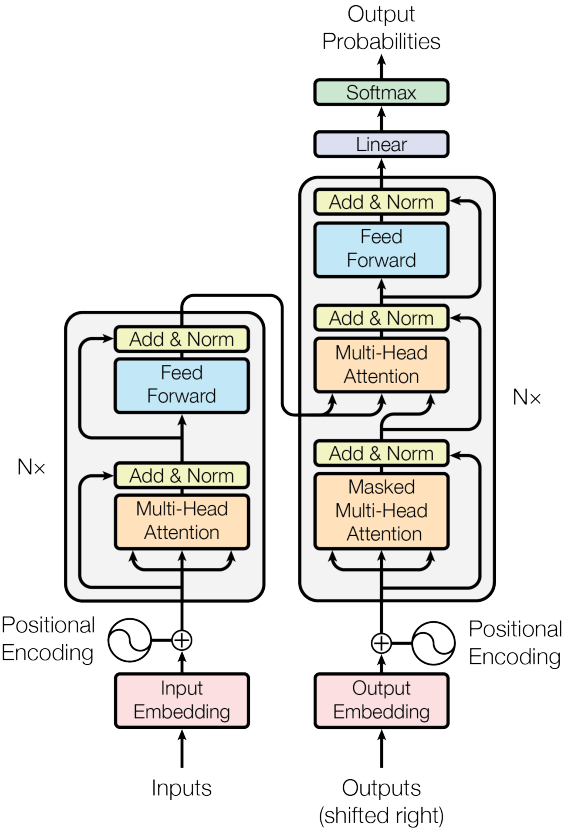
\includegraphics[width=0.4\textwidth]{theoretical-background/image/transformer.png}
    \caption{The architecture of transformers presented in the research paper "Attention is all you need" \cite{NIPS2017_3f5ee243}}
    \label{fig:transformer}
\end{figure}

\subsubsection{Vision Transformer}
After the fast development of Non-heritage model from LLMs, researcher tries to applied these structure for the Computer Visions. They have well performance in the Image Classifications compare to other Heritage Backbone Model at the time, however, Transformer still can not perform well on other computer vision tasks, such for Image Segmentations, and other main problem is the Quadrantic Complexity. 

Vanilla Vision Transformer is introduced back in 2021 to adapt attention in Computer Vision, figure \textbf{\ref{fig:vViT}}, that adapt input of Image patches of flattern image or their feature map with their corresponding encoding positions reshape the image x $\in$ R H×W×C into a sequence of flattened 2D patches ${x_p}$ $\in$  R N×$(P^2·C)$ , where (H, W) is the resolution of the original image, C is the number of channels, (P, P) is the resolution of each image patch, and N = HW/P2
is the resulting number of patches\cite{dosovitskiy2020image}

In Computer Vision, image having wider range of Variance and more en-rich data that can be captured than in LLMs systems, while Traditional Transformers focus on capturing most relationships between tokens through attention distributions, guided by fixed positional encodings, the most important information in high-dimenstion data is often be over-looked by the model itself, which can be struggle to capture local texture and edge informations. 

Researcher try to solve this problem through a more Spatial information enriched for the input before the Positional Encoding Staged, such as an adaptions for Laplacian-Former in a Laplacian pyramid or inputing the results of a Feature Map of CNN networks, in which can be computation costly and having high Fusion complexity, which can lets to mistaken information capture or over-lapped in non-relavent informations due to it's non-learnable feature extractions bias. 

\begin{figure}[h]
    \centering
    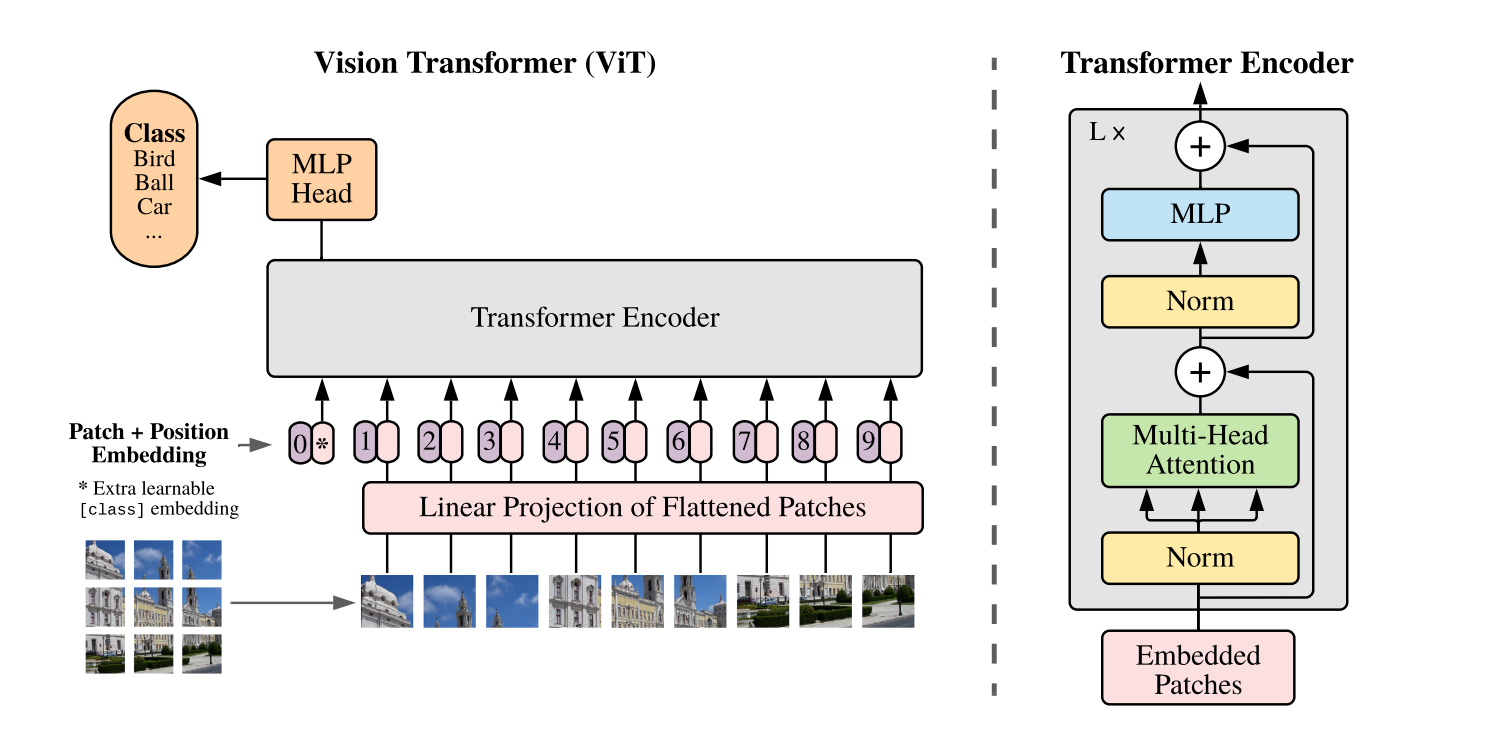
\includegraphics[width=0.75\linewidth]{theoretical-background/image/vanilaViT.png}
    \caption{Vanilla Vision-Transformer, \cite{dosovitskiy2020image}}
    \label{fig:vViT}
\end{figure}

\subsection{Heritage Model}
Heritage models such as \textbf{VGG} and \textbf{ResNet} have established foundational principles in convolutional neural network (CNN) design, achieving remarkable performance on large-scale image recognition tasks like ImageNet.

The \textbf{VGG} network, introduced by Simonyan and Zisserman~\cite{simonyan2014very}, is characterized by its deep and homogeneous architecture, constructed using stacks of $3 \times 3$ convolutional layers with fixed stride and padding. The simplicity of this design, along with increasing depth (e.g., 16 or 19 layers in VGG-16 and VGG-19), allows for the extraction of progressively more abstract visual features. However, the architecture incurs a high computational cost due to its large number of parameters, particularly in the fully connected layers. For example, VGG-16 contains approximately 138 million parameters, making it memory-intensive and less efficient for real-time applications.

In contrast, \textbf{ResNet} (Residual Network), introduced by He et al.~\cite{he2016deep}, enables the training of much deeper networks—e.g., ResNet-50, ResNet-101—by incorporating \emph{residual connections}. These skip connections allow the network to learn a residual mapping $F(\mathbf{x}) := H(\mathbf{x}) - \mathbf{x}$, where $H(\mathbf{x})$ is the desired underlying mapping and $\mathbf{x}$ is the input. The final output becomes:

\[
\mathbf{y} = F(\mathbf{x}) + \mathbf{x}
\]

This formulation helps combat the vanishing gradient problem by ensuring gradient flow through identity paths, allowing for deeper networks to be trained effectively. ResNet-50, for instance, has around 25 million parameters—substantially fewer than VGG-16—while achieving higher accuracy on standard benchmarks. This efficiency makes ResNet not only more scalable but also more computationally practical.  \cite{he2016deep}

Beyond VGG and ResNet, several other heritage models have introduced critical architectural innovations that influenced modern deep learning models in computer vision. One such concept is the \textbf{pyramid structure}, which enables effective multi-scale feature representation.

The \textbf{GoogLeNet} or \textit{Inception} architecture, proposed by Szegedy et al.~\cite{szegedy2015going}, introduced the Inception module that applies multiple convolutional operations in parallel—$1 \times 1$, $3 \times 3$, $5 \times 5$ convolutions, and max-pooling—and concatenates their outputs along the channel dimension. This design captures features at multiple receptive fields, enhancing the network’s ability to model information across scales. Moreover, the use of $1 \times 1$ convolutions as bottlenecks reduces dimensionality and computational cost, allowing the network to go deeper without an explosion in parameters.

The idea of building \textbf{feature pyramids} was later formalized in the \textbf{Feature Pyramid Network (FPN)}~\cite{lin2017feature}. FPN leverages the inherent hierarchical nature of CNNs to build a rich, multi-scale feature representation for tasks like object detection. Given a backbone feature extractor (e.g., ResNet), FPN constructs a top-down architecture with lateral connections, where high-level semantic features are upsampled and combined with lower-level features:

\[
P_l = \text{Conv1x1}(C_l) + \text{Upsample}(P_{l+1})
\]

Here, \( C_l \) denotes the feature map at level \( l \) from the backbone, and \( P_l \) is the corresponding pyramid output. This process ensures that each level in the pyramid contains both strong semantic and localization information, making it highly effective for detecting objects of different scales.

Another variation of the pyramid idea is the \textbf{Laplacian Pyramid Network}~\cite{denton2015deep}, which decomposes images into different frequency bands and processes each scale separately, a technique particularly useful in generative models.

\subsubsection{Attention Heritage model}

Transformers have demonstrated remarkable performance in natural language processing, and their adaptation to computer vision has spurred a range of novel architectures. The vanilla Vision Transformer (ViT) treats images as a sequence of fixed-size patches and applies global self-attention across all tokens. While effective for classification, this approach is limited in modeling hierarchical features and incurs high computational cost on high-resolution images.

To address these limitations, hierarchical Vision Transformers introduce a design that mimics the multi-scale feature extraction of CNNs. In this architecture, token representations are processed at increasingly coarser spatial resolutions as the network depth increases. Each stage reduces the spatial dimensions via patch merging while increasing the token embedding size. As a result, hierarchical Transformers can more efficiently capture fine-to-coarse image structures, making them suitable for dense prediction tasks such as detection and segmentation.
